% \chapter{Méthode LMI }
\chapter{Synthèse d'un retour statique de sortie par optimisation LMI}
\minitoc
\label{chap:LMI}

\section{Motivation}
\label{sec:motivationLMI}

Dans le chapitre précédemment, nous avons exploré la possibilité de stabiliser la dynamique longitudinale du drone à l'aide d'un contrôleur par retour dynamique de sortie. Les gains du contrôleur sont obtenus par une optimisation non-lisse basée sur des critères $H_{\infty}$. Nous proposons à présent d'étudier une manière différente de régler les gains du contrôleur, basée sur les inégalités linéaires matricielles.

Ce chapitre va permettre la mise en œuvre d'une formulation mathématique pour la synthèse du contrôleur basé modèle dans un cas pratique. Jusqu'à présent, cette approche a été testée et évaluée uniquement sur des cas théoriques \cite{Arzelier2018} avec des modèles dynamiques peu représentatif des systèmes réels. 

La méthode proposée pour contrôler le modèle de drone convertible étudié est basée sur la synthèse d'un contrôleur statique de sortie. 

La synthèse d'un contrôleur par retour de sortie statique pour la dynamique de DarkO augmentée s'inspire de \cite{SYRMOS1997125} où il est montré qu'un retour de sortie dynamique d'ordre $q \leq n$ (système d'ordre $n$), peut être converti en un retour de sortie statique à travers l'augmentation de l'espace d'état. Dans notre cas, des termes dynamiques tels que des intégrateurs et des filtres sont ajoutés à la dynamique du système, ce qui donne un espace d'état augmenté pour lequel une loi de bouclage statique composée d'une matrice de gain statique sera synthétisée.

La structure du correcteur permet de séparer  très clairement la partie dynamique représentée entre autres par l'intégrateur et la partie statique  qui est représentée par les matrices de gain $K$ et $H$. Dans le chapitre \ref{chap:3DOF}, les gains ont été obtenus par un outil d'optimisation non-lisse en se basant sur des contraintes fréquentielles $H_{\infty}$. Dans ce chapitre, on cherche à synthétiser $K$ et $H$ par un outil d'optimisation cette fois-ci convexe du type LMI pour un problème qui est originellement du type BMI, ce qui engendre nécessairement un certain conservatisme dans la solution.

Le contrôleur est obtenu en convertissant algorithmiquement le problème d'inégalités matricielles bilinéaires (BMI) non convexe en trois problèmes convexes auxiliaires :
\begin{itemize}
    \item un problème de retour d'état (SF),
    \item un problème d'injection de sortie (OI),
    \item un problème d'injection d'état (SI)
\end{itemize}

\nomenclature[]{\(BMI\)}{Inégalités matricielles bilinéaires  (\textit{Bilinear Matrix Inequalities})}
\nomenclature[]{\(SF\)}{Retour d'état  (\textit{State Feedback})}
\nomenclature[]{\(OI\)}{Injection de sortie (\textit{Output Injection})}
\nomenclature[]{\(SI\)}{Injection d'état (\textit{State injection})}


La résolution des problèmes (SF), (OI) et (SI) est une condition nécessaire à l'existence d'une solution pour le problème de retour statique de sortie. Par conséquent, la résolution de chacun des problèmes ci-dessus est abordée au moyen d'un algorithme en trois phases présenté à la section \ref{SOF Controller Synthesis}. Cet algorithme est mis en œuvre sur la dynamique augmentée de DarkO, laquelle est incorporée dans la boucle ouverte pour imposer une forme souhaitée semblable aux principes du \textit{loop shaping} \cite{McFarlane1992}. Cela conduit à des garanties multiples, notamment en termes de performance (avec un gain élevé en boucle ouverte à basse fréquence) et en termes de robustesse (avec une stratégie de gain faible en boucle ouverte à haute fréquence), tout en satisfaisant à l'exigence de suivi de la référence. 

Les contrôleurs par retour statique de sortie seront validés par des simulations dans le domaine temporel. De plus, une validation sera également effectuée de manière expérimentale par le biais d'essais en vol réels, avec un modèle expérimental du drone DarkO. 

Le chapitre est organisé comme suit. La section \ref{SOF Controller Synthesis} détaille l'algorithme itératif pour la conception des contrôleurs par retour statique de sortie, ainsi que le processus d'augmentation du système. Dans la section \ref{resultLMI}, les résultats de la synthèse du contrôleur sont analysés au moyen de simulations dans le domaine temporel et d'expérimentations, en mettant en œuvre les lois de contrôle conçues directement sur le système réel. 



\section{Synthèse d'un contrôleur statique de sortie}
\label{SOF Controller Synthesis}

La synthèse d'un contrôleur statique de sortie pose un problème non convexe en raison des multiplications entre les variables de décision, ce qui entraîne des inégalités matricielles bilinéaires (BMI). Cette complexité rend le problème d'optimisation NP-difficile. 
En se référant à la formulation des BMI dans \cite{ebihara2015}, plusieurs reformulations équivalentes sont proposées dans \cite{Arzelier2018}, ce qui conduit à l'inégalité matricielle présentée dans \eqref{MainMatrixIneq}. La méthode proposée ici est extraite de \cite{ebihara2015}, s'appuyant notamment sur l'approche S-variable et les calculs duaux.



\begin{equation}
\centering
  \begin{gathered}
        \textcolor{blue}{P} \succ 0 \\
        He\left\{ \smallmat{
            0 & 0 & \textcolor{blue}{P}\\
            0 & 0 & 0\\
            \textcolor{blue}{P} & 0 & 0
        }\right\}
    \prec
    He\left\{\smallmat{
        \mathbb{I}\\
            -\left( \textcolor{blue}{\lambda} \smallmat{
                C\\
                0_{p-n,n}                
            } + \textcolor{blue}{M} \right)\\
            -A
    }
    \textcolor{blue}{S_1} +
    \smallmat{
        0\\
        \textcolor{blue}{S_2}\\
        B\textcolor{blue}{Z}
    }
    \smallmat{
        0 & \mathbb{I} & -\textcolor{blue}{H}^T
    }\right\}
    \end{gathered}
    \label{MainMatrixIneq}
\end{equation}
\begin{equation}
    \boldsymbol{F} = -\textcolor{blue}{Z} \textcolor{blue}{S_2}^{-1} \smallmat{ \mathbb{I}_p \\ 0_{n-p,p} }
    \label{GetF}
\end{equation}

Même si cette nouvelle reformulation est toujours non-convexe, elle permet d'obtenir un résultat. Si une solution est trouvée pour le système dans \eqref{MainMatrixIneq} avec $\textcolor{blue}{\lambda} = 1$, $\textcolor{blue}{M} = 0$ et $\textcolor{blue}{S_2}$ non singulière, alors nous pouvons calculer une matrice de gain $\boldsymbol{F}$ qui garantit la stabilité en boucle fermée (la preuve est disponible dans \cite{Arzelier2018}). Cette matrice de gain, qui n'est pas directement optimisée dans la synthèse convexe, est obtenue à l'aide de \eqref{GetF}. 

Cette preuve constitue l'objectif principal du processus d'optimisation. Relever les défis découlant de la nature non convexe du problème \ref{MainMatrixIneq} nécessite des développements mathématiques et techniques spécifiques. La formulation mathématique introduite dans la littérature a donné des résultats théoriques initiaux prometteurs. L'algorithme, qui sera détaillé dans la sous-section suivante, sera appliqué à la dynamique du drone DarkO. L'analyse qui en résultera permettra de tirer des conclusions quant à l'efficacité de l'algorithme dans des scénarios d'essai pratiques.


\subsection{Algorithme itératif pour la conception de retour statique de sortie}
\label{3a}

Le problème de la synthèse de gain d'un retour statique de sortie se caractérise par sa nature intrinsèquement non convexe qui s'accompagne de difficultés de calcul liées aux problèmes NP-difficile. Ceci, associé à une complexité inhérente qui provient de l'impossibilité d'optimiser toutes les variables de décision simultanément, rend le processus de division du problème non-convexe en de multiples sous-problèmes convexes auxiliaires extrêmement attrayant. L'inégalité matricielle bilinéaire \eqref{MainMatrixIneq} sera utilisée pour traduire ces objectifs dans un cadre d'optimisation. Chaque objectif particulier est atteint en fixant de manière optimale une partie des variables de décision, tout en affinant le reste par un processus itératif. Pour concevoir le contrôleur, un algorithme en trois phases introduit dans \cite{Arzelier2018} sera mis en œuvre Fig. \ref{AlgoPhases}, lequel prend en entrée les matrices $\boldsymbol{A}$, $\boldsymbol{B}$, $\boldsymbol{C}$ de la dynamique linéarisée du système.

\begin{figure}[hbt]
    \centering
      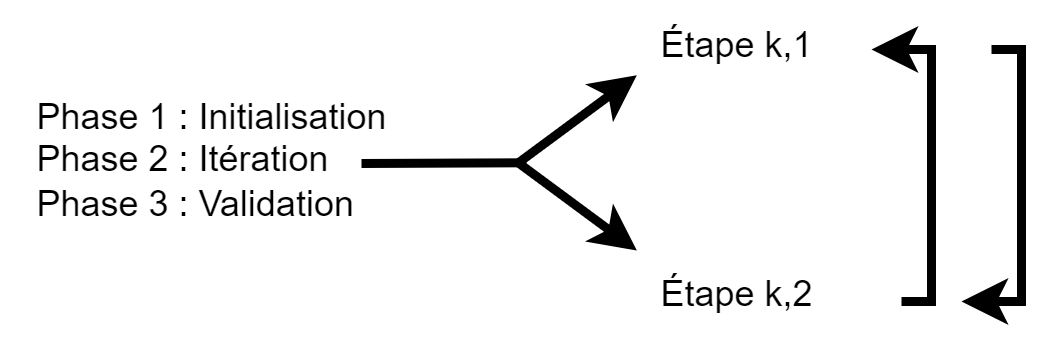
\includegraphics[width=0.6\columnwidth]{figures/LMIAlgo.png}
      \vspace{-0.2cm}\caption{Structure de l'algorithme d'optimisation.}
      \label{AlgoPhases}
\end{figure} 

\subsubsection{Phase d'initialisation} 
L'objectif de la première phase est essentiellement de fournir une estimation initiale pour un contrôleur matriciel de gain à retour d'état $\boldsymbol{K}$ qui stabilise la boucle fermée $\dot{\boldsymbol{x}}=(\boldsymbol{A}+\boldsymbol{B}\boldsymbol{K})\boldsymbol{x}$. Pour ce faire, la stratégie adoptée consiste à fixer les variables de décision \textcolor{blue}{$\lambda$, M, H} de \eqref{MainMatrixIneq} de la manière suivante :
\begin{equation}
    \begin{gathered}
        \textcolor{blue}{\lambda} = \lambda = 0, \quad
        \textcolor{blue}{M} = M_0 = \begin{pmatrix}
            C^{\circ}C\\
            {C^{\perp}}^T
        \end{pmatrix},\\
        \textcolor{blue}{H} = H_0 = J M_0^{-1}, \quad
        J = (-\mu-h)\mathbb{I},
    \end{gathered}
    \label{InitVariableFixing}
\end{equation} 
où $h$ est un scalaire positif et $-\mu$ est la partie réelle maximale des valeurs propres de $\boldsymbol{A}$. L'étude de faisabilité menée dans la phase d'initialisation est la suivante :

\begin{equation}
    \begin{gathered}
        \textcolor{blue}{P} \succ 0 \\
        He\left\{ \smallmat{
            0 & 0 & \textcolor{blue}{P}\\
            0 & 0 & 0\\
            \textcolor{blue}{P} & 0 & 0
       }\right\}
    \prec
    He\left\{\smallmat{
        \mathbb{I}\\
            -M_0 \\
            -\boldsymbol{A}
   }
    \textcolor{blue}{S_1} +
    \smallmat{
        0\\
        \textcolor{blue}{S_2}\\
        B\textcolor{blue}{Z}
    }
    \smallmat{
        0 & \mathbb{I} & -H_0^T
    }\right\}
    \end{gathered}
    \label{InitMatrixIneq} 
\end{equation} 

Si \eqref{InitMatrixIneq} est réalisable pour une combinaison de variables de décision \textcolor{blue}{$S_1$, $S_2$, Z} et pour le certificat de Lyapunov \textcolor{blue}{P}, alors une première estimation d'un gain de retour d'état stabilisant $\boldsymbol{K}$ est trouvée, et nous pouvons passer à la phase d'itération. En revanche, si aucune solution n'est trouvée, le paramètre $h$ est incrémenté de 1 et la phase d'initialisation est exécutée à nouveau. Cette phase résout les problèmes (SI) et (SF). Les résultats de cette phase sont les suivants :

\begin{equation}
    \begin{gathered}
        S_{1.0}=\textcolor{blue}{S_1},  \quad
        \hat{K}_0 = -\textcolor{blue}{Z} \textcolor{blue}{S_2}^{-1}, \quad
        K = -\textcolor{blue}{Z} \textcolor{blue}{S_2}^{-1} M_0
    \end{gathered}
    \label{OutputsInit}
\end{equation}

\subsubsection{Phase d'itération - Étape k,1}

Cette phase comprend deux étapes itératives. Dans la première étape, les variables d'optimisation $\lambda$ et $\boldsymbol{M}$ dans \ref{MainMatrixIneq} précédemment fixées lors de l'initialisation, sont maintenant traitées comme des variables de décision. Pour maintenir la convexité; la variable de marge \textcolor{blue}{$S_1$} est fixée à la valeur $S_{1,0}$ déterminée lors de la phase d'initialisation. Le système \eqref{Iter1MatrixIneq} est ensuite résolu.

\begin{equation}
\centering
    \begin{gathered}
        \textcolor{blue}{P} \succ 0, \quad \smallmat{
            (1-\textcolor{blue}{\lambda})\mathbb{I} & \textcolor{blue}{M^T}\\
            \textcolor{blue}{M} & \mathbb{I}
        } \geq 0 ,\quad \textcolor{blue}{\lambda} \geq 0 \\
        He\left\{ \smallmat{
            0 & 0 & \textcolor{blue}{P}\\
            0 & 0 & 0\\
            \textcolor{blue}{P} & 0 & 0
        }\right\}
    \prec
    He\left\{\smallmat{
            \mathbb{I}\\
            -\left( \textcolor{blue}{\lambda}
            \smallmat{
                C\\
                0_{p-n,n}
             } +
            \textcolor{blue}{M}
            \right) \\
            -A
    }
    S_{1,k-1} +
    \smallmat{
         0\\
        -\mathbb{I}\\
        B \hat{K}_{k-1}
    }
    \smallmat{
        0 & -\textcolor{blue}{S_2} & \textcolor{blue}{Y}^T
    }\right\}
    \end{gathered}
    \label{Iter1MatrixIneq}
\end{equation}

Dans \eqref{Iter1MatrixIneq}, deux inégalités matricielles apparaissent en plus de l'inégalité du certificat de Lyapunov et de l'inégalité \eqref{MainMatrixIneq}. Ces contraintes supplémentaires contribuent à la réalisation de l'objectif de la phase d'itération, qui consiste à trouver une solution pour \eqref{MainMatrixIneq} dans laquelle les variables $\lambda$ et $\boldsymbol{M}$ convergent respectivement vers 1 et 0, ce qui est une condition obligatoire pour atteindre l'objectif d'optimisation principal. Pour ce faire, la maximisation de $\lambda$ est définie comme un objectif dans le solveur d'optimisation. Une inégalité matricielle contraint la norme de $\boldsymbol{M}$ et la réduit à 0, à mesure que $\lambda$ augmente jusqu'à 1. La seconde inégalité est simplement une contrainte sur $\lambda$, ce dernier devant être positif.


Si une solution est trouvée pour \eqref{Iter1MatrixIneq} et si, pour cette solution, $1-\lambda$ est inférieur à une tolérance définie, cela signifie que l'on peut passer à la troisième et dernière phase, à savoir la validation. Les résultats de cette phase sont les suivants :

\begin{equation}
    \begin{gathered}
        \lambda_k=\textcolor{blue}{\lambda},  \quad
        M_k = \textcolor{blue}{M}, \quad
        H_k^T = \textcolor{blue}{S_2}^{-1} \textcolor{blue}{Y}^T
    \end{gathered}
    \label{OutputsIterStap2}
\end{equation}

Si ce n'est pas le cas, il y a une deuxième étape dans la phase d'itération.

\subsubsection{Phase d'itération - Étape k,2}


L'étape k,2 est relativement proche d'une étape d'initialisation. Comme pour la première phase, où \textcolor{blue}{$\lambda$, $M$} et \textcolor{blue}{$H$} ont été fixés comme entrées pour générer un gain de retour d'état stabilisateur $\boldsymbol{K}$, la deuxième étape fixe les mêmes variables de décision avec des valeurs mises à jour à partir de l'étape k,1.

Le problème d'optimisation à résoudre dans cette phase est le suivant :


\begin{equation}
\centering
    \begin{gathered}
        \textcolor{blue}{P} \succ 0 \\
        He\left\{ \begin{bmatrix}
            0 & 0 & \textcolor{blue}{P}\\
            0 & 0 & 0\\
            \textcolor{blue}{P} & 0 & 0
        \end{bmatrix}\right\}
    \prec
    He\left\{\begin{bmatrix}
           \mathbb{I}\\
                -\hat{M}(\textcolor{blue}{\alpha})\\
            -A
    \end{bmatrix}
    \textcolor{blue}{S_1} +
    \begin{bmatrix}
        0\\
        \textcolor{blue}{S_2}\\
        B\textcolor{blue}{Z}
    \end{bmatrix}
    \begin{bmatrix}
        0 & \mathbb{I} & -H_k^T
    \end{bmatrix}\right\}
    \end{gathered}
    \label{Iter2MatrixIneq}
\end{equation}
\begin{equation}
    \begin{gathered}
        \hat{M}(\textcolor{blue}{\alpha}) = \left((1+\textcolor{blue}{\alpha} (\lambda_k-1))
        \begin{bmatrix}
            C \\
            0_{p-n,n}
        \end{bmatrix}
        +
        \textcolor{blue}{\alpha} M_k\right)
    \end{gathered}
    \label{Artificiu2}
\end{equation}

Lors de cette étape, un nouveau terme, $\hat{M}(\textcolor{blue}{\alpha})$ apparaît, dépendant d'une nouvelle variable de décision $\textcolor{blue}{\alpha}$. L'objectif est de minimiser \textcolor{blue}{$\alpha$} à l'aide de la méthode de bissection, en convertissant le problème non convexe en un problème convexe. Idéalement, \textcolor{blue}{$\alpha$} converge vers 0, signalant la fin de cette phase d'itération et la progression vers la phase de validation finale. Si $\alpha \approx 0$ selon une certaine tolérance, \eqref{Artificiu2} se simplifie en \eqref{Artificiu3}. Par conséquent, les valeurs des variables de décision pour la solution de \eqref{Iter2MatrixIneq} lors l'étape k,2 sont identiques à la solution de \eqref{MainMatrixIneq}, laquelle est résolue pour $\lambda = 1$ et $\boldsymbol{M} =0$. Cette solution permet le calcul d'un contrôleur par retour de sortie statique stabilisant.

\begin{equation}
    \begin{gathered}
        \hat{M}(\alpha) = \left((1+\alpha (\lambda_k-1))
        \begin{bmatrix}
            C \\
            0_{p-n,n}
        \end{bmatrix}
        + 
        \alpha M_k\right)
        \stackrel{\alpha \approx 0 }{=}
        \begin{bmatrix}
            C \\
            0_{p-n,n}
        \end{bmatrix}
    \end{gathered}
    \label{Artificiu3}
\end{equation}

Si, à l'étape k,2, $\alpha$ n'est pas inférieure à la tolérance fixée, l'algorithme commence une nouvelle étape d'itération à k,1. Les résultats de la phase actuelle sont les suivants :

\begin{equation}
    \begin{gathered}
\alpha_k=\textcolor{blue}{\alpha}  \quad
        \hat{K}_{k-1} = -\textcolor{blue}{Z} \textcolor{blue}{S_2}^{-1} \quad
        S_{1,k} = \textcolor{blue}{S_1}
    \end{gathered}
    \label{OutputsIterStap1}
\end{equation}

\subsubsection{Phase de validation}
Dans les cas où l'étape d'itération fournit une solution pour laquelle $\boldsymbol{\lambda} = 1 $ et $\boldsymbol{M} = 0$, une phase de validation n'est pas nécessaire car le contrôleur peut être calculé directement. 

En pratique, l'algorithme quitte la phase d'itération avec des solutions $\boldsymbol{\lambda} \approx 1$ et $\boldsymbol{M} \approx 0$, en raison des limites des solveurs d'optimisation et des précisions numériques. Dans ces cas, les conditions pour atteindre l'objectif d'optimisation principal ne sont pas exactement remplies. Par conséquent, une phase de validation est nécessaire. Le problème à résoudre est défini par \eqref{ValidMatrixIneq}, où les variables sont fixées $\boldsymbol{\lambda} = 1$ et $\boldsymbol{M} = 0$ et $\boldsymbol{H}$ est fixé à $\boldsymbol{H_k}$ (obtenu au cours de la phase d'itération).
Si l'inégalité \eqref{ValidMatrixIneq} est satisfaite alors la matrice de gain $\boldsymbol{F}$ peut être construite avec \eqref{GetF}, ce qui garantit la stabilité la boucle fermée $(\boldsymbol{A}+\boldsymbol{B}\boldsymbol{F}\boldsymbol{C})$. Cette dernière phase fournit la solution aux objectifs (OI) et (OF). 

\begin{equation}
\centering
    \begin{gathered}
        \textcolor{blue}{P} \succ 0 \\
        He\left\{ \begin{bmatrix}
            0 & 0 & \textcolor{blue}{P}\\
            0 & 0 & 0\\
            \textcolor{blue}{P} & 0 & 0
        \end{bmatrix}\right\}
    \prec
    He\left\{\begin{bmatrix}
            \mathbb{I}\\
                -\begin{bmatrix}
                    C \\
                    0_{p-n,n}
                \end{bmatrix}\\
            -A
    \end{bmatrix}
    \textcolor{blue}{S_1} +
    \begin{bmatrix}
        0\\
        \textcolor{blue}{S_2}\\
        B\textcolor{blue}{Z}
    \end{bmatrix}
    \begin{bmatrix}
        0 & \mathbb{I} & -H^T
    \end{bmatrix}\right\}
    \end{gathered}
    \label{ValidMatrixIneq}
\end{equation}


\subsection{Architecture de commande}
\label{3b}


L'architecture de contrôle du drone DarkO est conçue pour le stabiliser en vol stationnaire, avec et sans perturbations externes. Par exemple, pour contrer un vent de face affectant la vitesse linéaire le long des axes $x_{[b]}$ et $z_{[b]}$ et générant un moment autour de l'axe $y_{[b]}$, le schéma de commande utilise les ailerons et les hélices de manière symétrique pour générer un moment et une force compensatoires. Une action intégrale est employée pour contre-balancer la force le long de l'axe $z_{[b]}$, assurant une convergence asymptotique vers la force désirée en utilisant deux intégrateurs, un pour les moteurs et un pour les élevons.


 L'architecture mise en œuvre, présentée à la figure \ref{Plant Augmentation}, est une reformulation de la loi de contrôle présentée dans le chapitre \ref{chap:3DOF}. Elle se compose du bloc dynamique linéarisé du drone DarkO \eqref{eq:linearized} avec les matrices $\boldsymbol{A}_{0}$ \eqref{matrice_A} et $\boldsymbol{G}_{0}$ \eqref{matriceG0}, du bloc de saturation pour les deux hélices et les deux élevons, comme présenté dans la section \ref{sec:saturation}. La matrice de sélection des sorties élimine la mesure de l'état de l'angle de tangage, $\theta$.

\begin{figure}[hbt]
    \centering
    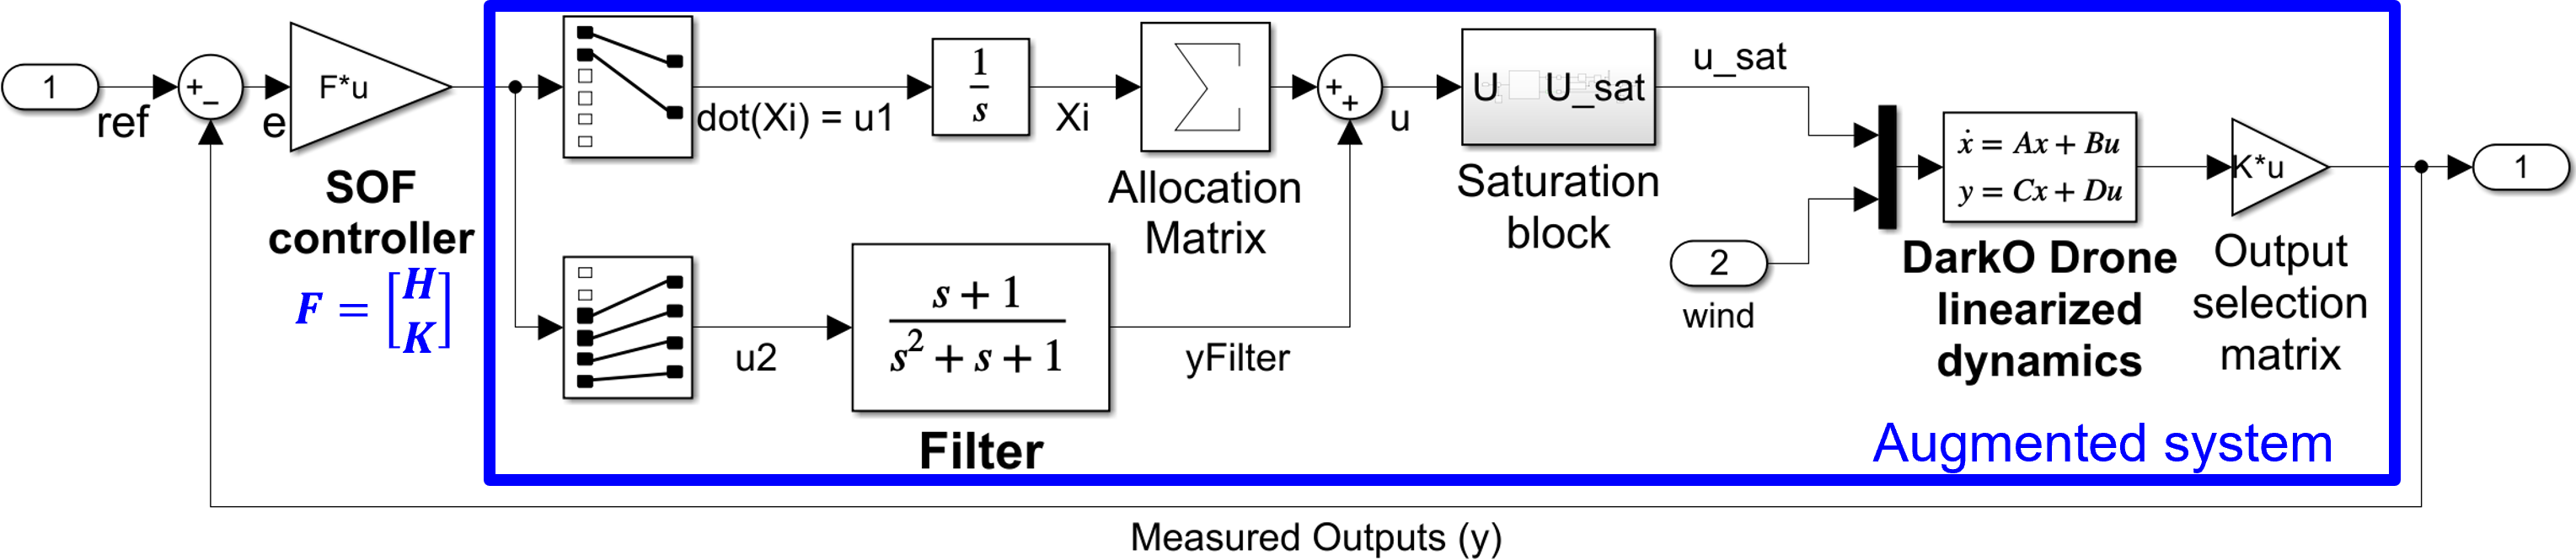
\includegraphics[width=0.9\columnwidth]{figures/AugWindFinal.png}
    \vspace{-0.3cm}\caption{Augmentation du système.}
    \label{Plant Augmentation}
\end{figure}


Pour la conception du contrôle, une structure de contrôleur de type PI est employée pour minimiser l'erreur statique et améliorer le rejet des perturbations externes. Pour ce faire, nous ajoutons des filtres pré-compensateurs à l'entrée du système, sur la base de la méthodologie de \textit{loop shaping}. Un intégrateur est ajouté pour assurer la performance (gain élevé) à basse fréquence, ce qui correspond à la spécification de suivi. De même, un filtre de deuxième ordre est ajouté pour assurer que le contrôleur soit strictement propre et robuste en ce qui concerne les dynamiques négligées grâce à un comportement d'atténuation. La fréquence de coupure du filtre est fixée à environ \SI{5}{\hertz} pour s'aligner sur la dynamique de la boucle fermée et rejeter le bruit dans les signaux mesurés. Pour limiter le nombre d'intégrateurs à 2 (un qui génère la commande d'intégration pour les deux hélices et l'autre pour les deux élevons), les sorties du bloc intégrateur sont doublées par une matrice d'allocation $\Sigma$. L'implémentation d'un filtre de second ordre présente l'avantage supplémentaire d'éviter un terme de transmission directe, qui peut amplifier les bruits de mesure indésirables sur $\boldsymbol{y}$ et qui se répercute sur les capteurs. La matrice de gain $\boldsymbol{F}$ comprend les matrices de gain $\boldsymbol{H}$ et $\boldsymbol{K}$ respectivement pour l'action intégrale et proportionnelle. Les équations et la représentation de l'espace d'état du système augmentée se trouvent dans \eqref{AugEq1}.

\begin{equation}
\centering
    \begin{gathered}
        \dot{x}_i = u_1, \\
        u = \Sigma x_i + y_{filter} = \Sigma x_i + Filter \cdot u_2 \\
        \dot{x} = Ax + Bu = Ax + B(\Sigma x_i + y_{filter}) = Ax + B\Sigma x_i + B C x_{filter}, \\
        \Sigma =
        \smallmat{
            1 & 0 \\ 1 & 0 \\ 0 & 1 \\ 0 & 1   
        }, \quad \quad
        \smallmat{
            u_1 \\ u_2   
        }
        = F e = F \left(\smallmat{ref \\ \mathbb{0}_{8\times 1} }-y\right)  ,\\
        \smallmat{
            \dot{x} \\ \dot{x_c} \\ \dot{x}_{filter}
        } =
        \smallmat{
            A & B \Sigma & B C_{filter} \\
            0 & 0 & 0 \\
            0 & 0 & A_{filter} 
        }
        \smallmat{
            x \\ x_c \\ x_{filter}
        }
        +
        \smallmat{
            0 & 0 \\ 1 & 0 \\ 0 & B_{filter}
        }
        \smallmat{
            u_1 \\ u_2
        },  \\
        y = \smallmat{
            C & 0 & 0
        }
        \smallmat{
            x \\ x_c \\ x_{filter}
        },
    \end{gathered}
    \label{AugEq1}
\end{equation}
où $\boldsymbol{x_i} \in \mathbb{R}^{2}$ sont les états des intégrateurs,  $\boldsymbol{x_f} \in \mathbb{R}^{4}$ sont les états des filtres, $\boldsymbol{r} \in \mathbb{R}^{3}$ est le signal de référence, $\boldsymbol{y} \in \mathbb{R}^{11}$ est la sortie mesurée et $\boldsymbol{u}\in \mathbb{R}^{4}$ est l'entrée du système.

\section{Résultats}
\label{resultLMI}
\subsection{Résultats de simulation}

L'approche de la section \ref{3a} a été appliquée au système augmenté de la section \ref{3b}, en se concentrant sur la dynamique linéarisée pour une vitesse de vent nulle (scénario de vol stationnaire). On a ainsi obtenu quatre contrôleurs stabilisateurs pour $h=12, 13, 14 \text{ et } 15$, $h$ variant entre 1 et 40. Plusieurs itérations avec différentes valeurs de $h$, servant de points d'initialisation pour l'algorithme d'optimisation, sont nécessaires pour améliorer la probabilité de convergence.

La figure \ref{HKStepRes_a} montre la réponse temporelle en boucle fermée des quatre contrôleurs, avec des variations de consigne sur l'axe $x$ à 5 s, l'axe $y$ à 70 s et l'axe $z$ à 40 s. Tous les contrôleurs stabilisent efficacement la dynamique en boucle fermée et suivent les références de position selon les trois axes. La réponse est lente sur les axes $x$ et $z$ et rapide sur l'axe $y$. Cela est dû à la capacité d'actionnement et l'utilisation différentielle des moteurs. De plus, une variation de consigne sur un axe n'entraîne pas de changement significatif sur les deux autres axes, ce qui indique un fort découplage entre les états de position. En outre, les actionneurs n'ont jamais été saturés.


\begin{figure}[hbt]
    \centering
   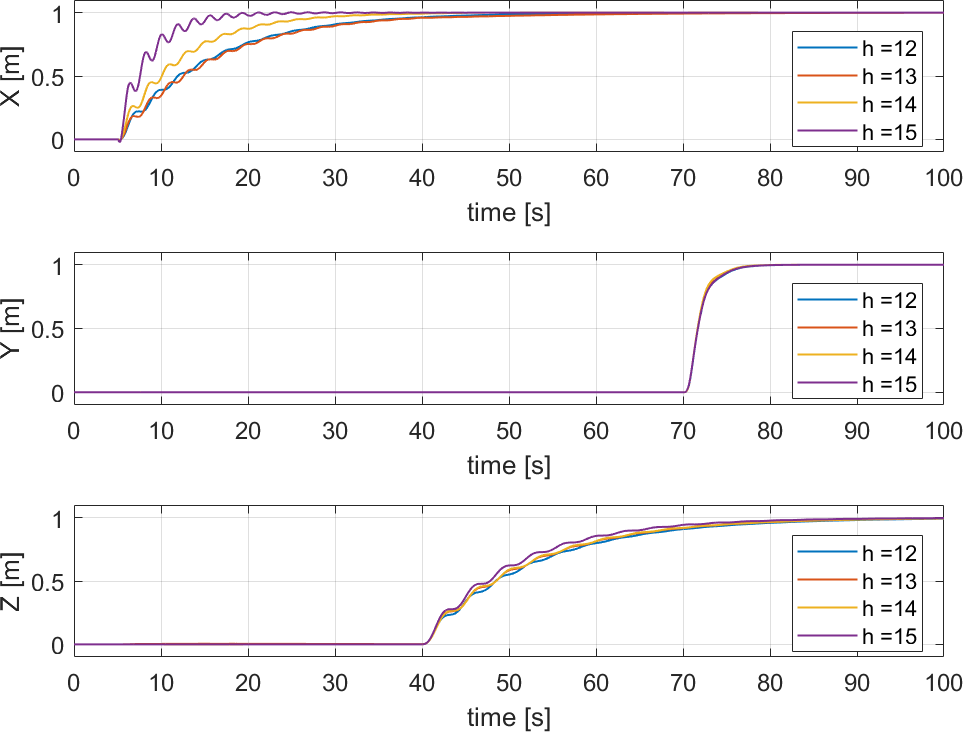
\includegraphics[width=0.7\columnwidth]{figures/stepResponse.png}
    \caption{Réponse du bouclage \eqref{AugEq1} avec une dynamique linéaire \eqref{eq:linearized}.}
    \label{HKStepRes_a}
\end{figure}

Le premier graphique de la figure \ref{thetanowind} montre que l'angle d'incidence $\theta$ subit des oscillations croissantes au fur et à mesure que h augmente. Bien que l'angle d'incidence $\theta$ ne soit pas directement contrôlé, il converge naturellement vers 0 lorsque les autres états se stabilisent, ce qui indique un vol stationnaire sans vent. Le second graphique montre que pour une dynamique linéarisée autour d'une vitesse de vent spécifique, $\theta$ converge vers une valeur non nulle, compensant les perturbations externes.

\begin{figure}[hbt]
    \centering
    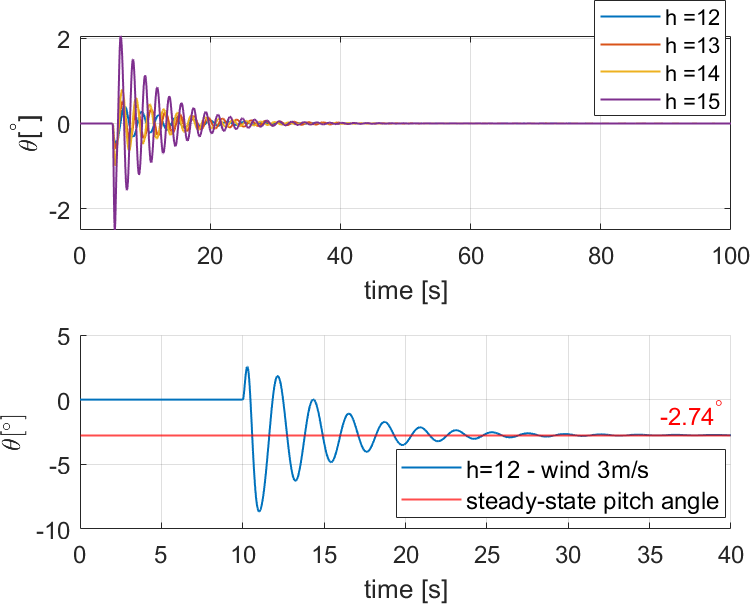
\includegraphics[width=0.7\columnwidth]{figures/windThetafinalhopeCrop.png}
    \vspace{-0.3cm}\caption{Réponse temporelle de l'angle d'incidence $\theta$ en boucle fermée.}
    \label{thetanowind}
\end{figure}

Les équations \eqref{Kstructure1} et \eqref{Kstructure2} présentent les gains du contrôleur synthétisés $\boldsymbol{F}$ (bloc illustré dans \ref{Plant Augmentation}) comprenant les gains matriciels $\boldsymbol{H}$ et $\boldsymbol{K}$ pour h=12 et une dynamique linéarisée à une vitesse de vent nulle. En examinant plus attentivement la matrice de gain $\boldsymbol{K}$ qui produit quatre signaux de commande utilisés pour la commande asymétrique ou symétrique des actionneurs du drone, on peut observer que les lignes 1 et 2 (qui génèrent une commande de poussée sur les deux hélices) ainsi que les lignes 3 et 4 (qui génèrent une commande d'angle de déflexion pour les deux élevons) sont soit presque égales, soit opposées, à quelques exceptions près. Ce modèle a émergé naturellement du processus d'optimisation sans aucune contrainte, reflétant un alignement intuitif et cohérent avec la dynamique du drone.

\begin{equation}\label{Kstructure1}
\boldsymbol{H}=
\smallmat{
  3.5e\shortminus6 & \shortminus3.0e\shortminus7 &  1.5e\shortminus2 & \shortminus6.9e\shortminus6 & \shortminus7.4e\shortminus6 &  4.4e\shortminus1 & 1.8e\shortminus4 &  1.1e\shortminus4 & \shortminus8.4e\shortminus5 & \shortminus8.6e\shortminus5 & \shortminus2.3e\shortminus4\\
  \shortminus2.0e\shortminus2 & \shortminus7.5e\shortminus6 &  1.6e\shortminus5 & \shortminus2.0e\shortminus1 &  4.4e\shortminus5 & \shortminus1.1e\shortminus4 & \shortminus9.2e\shortminus5 & \shortminus9.1e\shortminus5 &  7.4e\shortminus6 &  7.6e\shortminus1 & \shortminus3.9e\shortminus5}
\end{equation}
 \begin{equation}\label{Kstructure2}
\boldsymbol{K}=
\smallmat{
  7.6e\shortminus3 & \shortminus2.0e+1 &  9.9 &  3.1e\shortminus2 & \shortminus4.5e+1 &  8.2e+1 &\shortminus3.1e+2 & \shortminus3.1e+2 &  6.4e\shortminus1 &  3.0e\shortminus3 & \shortminus1.0e+2 \\
  5.4e\shortminus3 &  2.0e+1 &  9.9 &  8.8e\shortminus3 &  4.5e+1 &  8.2e+1 & 3.1e+2 &  3.1e+2 & \shortminus6.5e\shortminus1 & \shortminus1.9e\shortminus3 &  1.0e+2\\
  \shortminus4.2 & \shortminus3.2e\shortminus1 &  8.7e\shortminus3 & \shortminus4.5e+1 & \shortminus4.4e\shortminus1 & \shortminus3.1e\shortminus2 & \shortminus1.2e+1 &  1.6 & \shortminus3.1e+1 &  3.9e+1 & \shortminus1.6 \\
  \shortminus4.2 &  3.2e\shortminus1 &  4.8e\shortminus3 & \shortminus4.5e+1 &  4.3e\shortminus1 &  3.3e\shortminus2 & 1.2e+1 & \shortminus1.7 &  3.1e+1 &  3.9e+1 &  1.6}
\end{equation}



\subsection{Résultats expérimentaux}

Pour la validation expérimentale, les contrôleurs ont été testés sur le modèle réel de drone DarkO construit à l'ENAC Fig. \ref{DarkO1}. Les essais en vol ont eu lieu dans la volière de l'ENAC, équipée d'un système de capture de mouvement Optitrack fournissant des données de position et d'attitude à \SI{40}{\hertz}, éliminant ainsi le besoin d'un capteur GPS. La vitesse est obtenue par une différence finie. Des algorithmes de fusion de données, y compris des filtres invariants, ont combiné les données d'Optitrack (position, vitesse et attitude) et de l'unité IMU du drone DarkO pour améliorer l'estimation de l'état. Cette estimation est utilisée pour créer le vecteur de sortie $\boldsymbol{y}$, entrée de la loi de contrôle \eqref{AugEq1}. Compte tenu de l'architecture de la boucle de contrôle, l'estimation doit être de très bonne qualité avec le délai le plus court possible.

La nature modulaire de Paparazzi permet d'utiliser l'implémentation existante du filtre invariant pour estimer le vecteur d'état de DarkO et d'ajouter un module de stabilisation basé sur la loi de contrôle décrite ci-dessus (voir \ref{3b}). L'autopilote échantillonne les lois de commande et de contrôle à \SI{500}{\hertz}, générant des commandes de contrôle appropriées pour réaliser les manœuvres de vol souhaitées et stocker toutes les données en vue d'une analyse a posteriori.

\begin{figure}[ht]
    \centering
    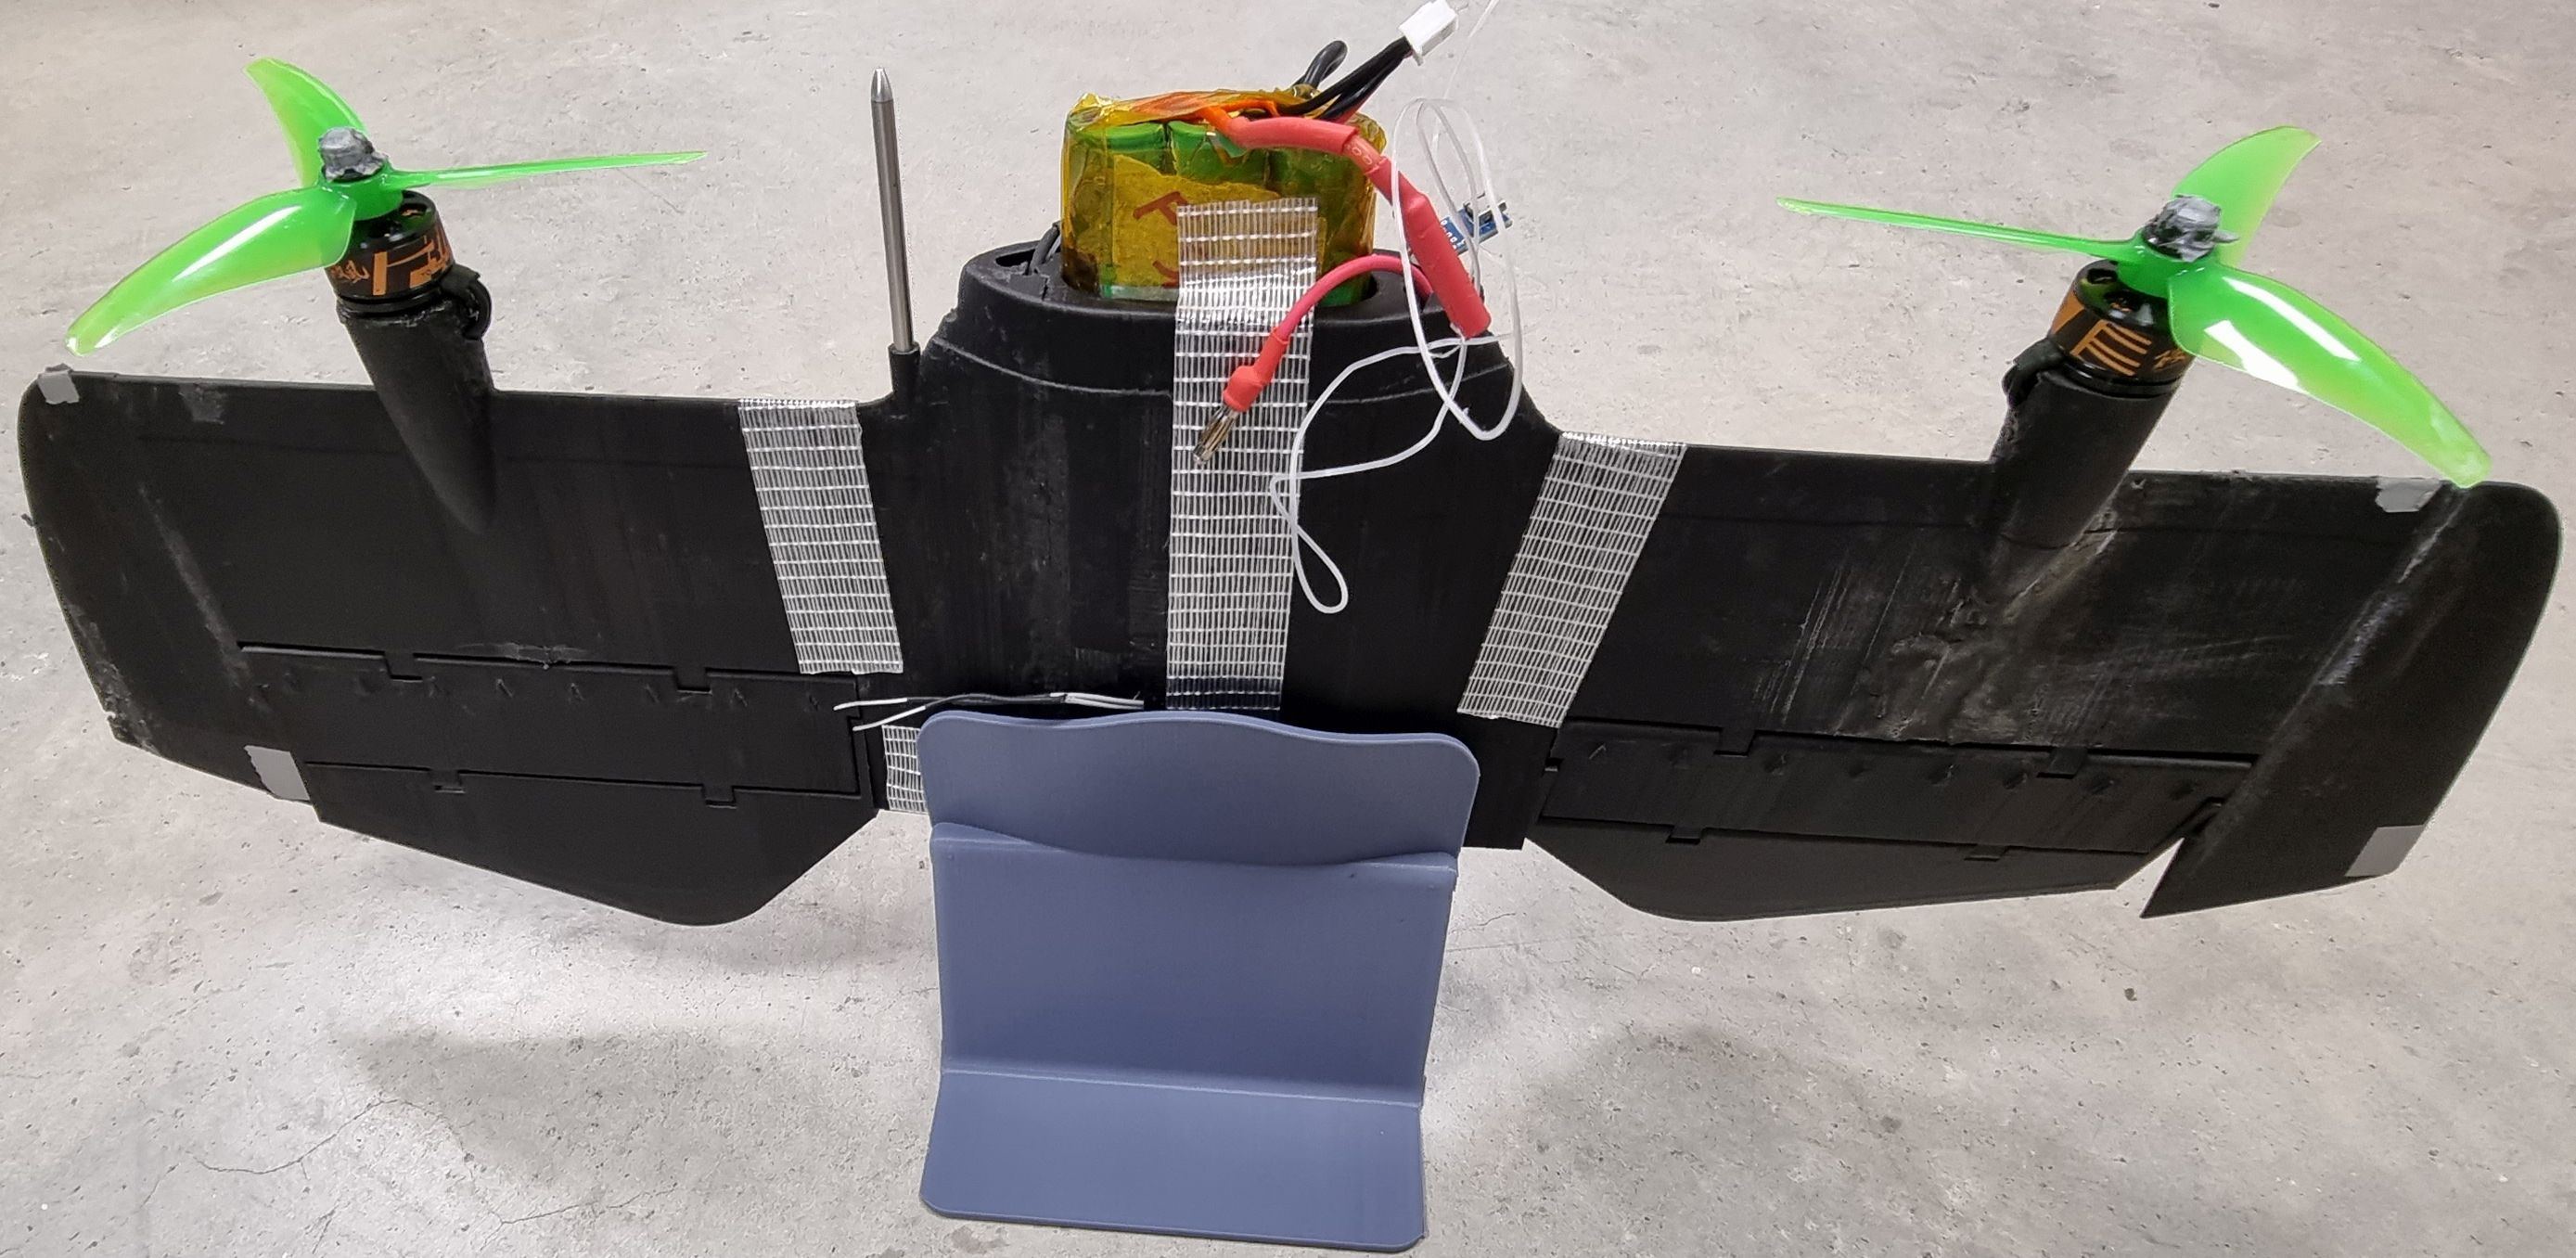
\includegraphics[width=0.7\columnwidth]{figures/DarkOModelfinal.jpg}
   \vspace{-0.2cm}\caption{Modèle expérimental du drone DarkO.}
    \label{DarkO1}
\end{figure}
\begin{figure}[ht]
    \centering
    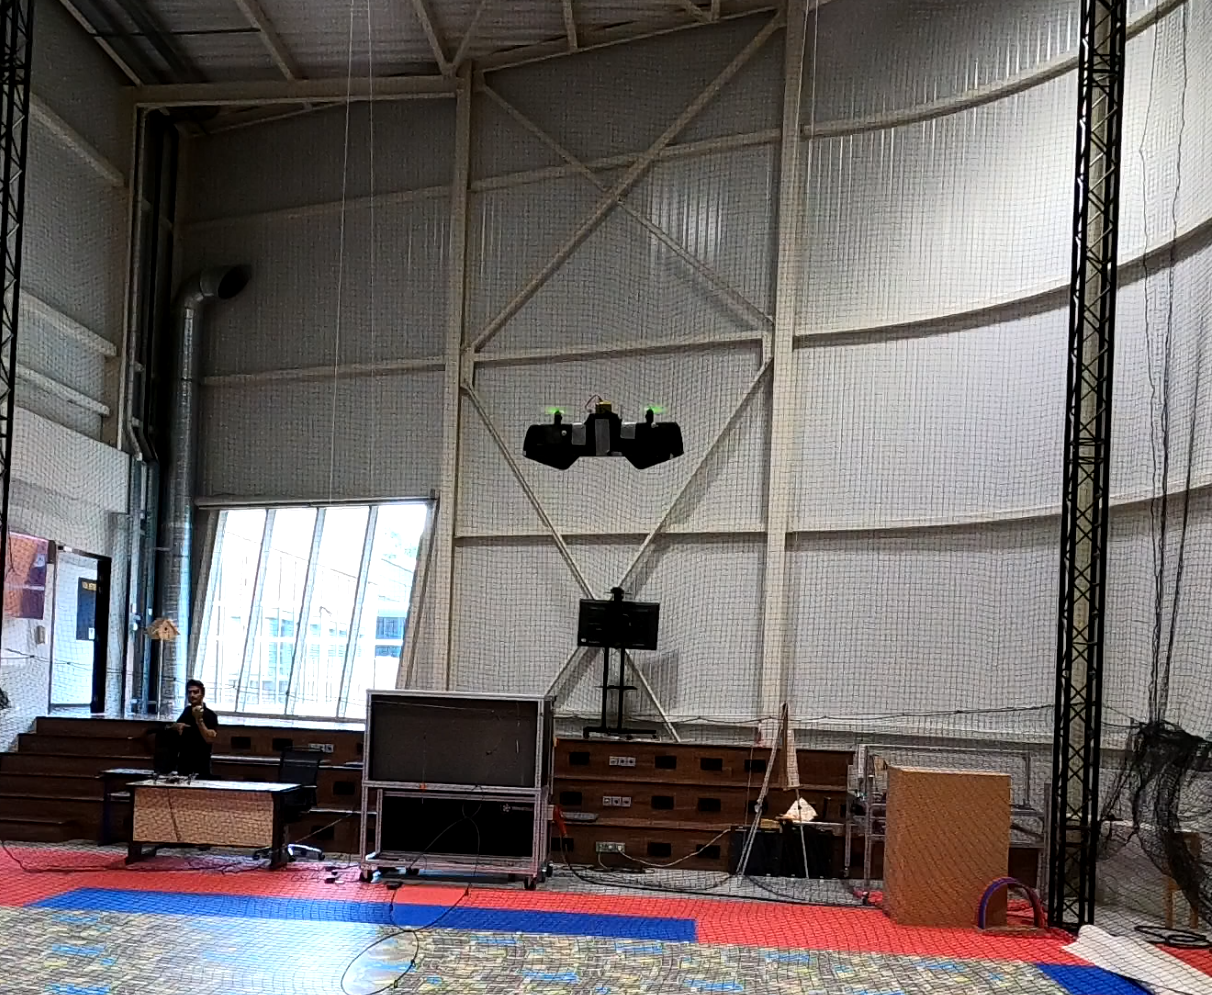
\includegraphics[width=0.8\columnwidth]{figures/DarkOFlighthope.png}
    \vspace{-0.2cm}\caption{DarkO lors d'un vol expérimental.}
    \label{DarkO2}
\end{figure}

Les essais expérimentaux suivants constituent les expérimentations réalisées dans la volière de l'ENAC où des contrôleurs ont été obtenu avec des méthodes de synthèse basées sur une modélisation du drone convertible. Les vols précédents pour ce type de drone utilisaient des conceptions de contrôle combinées basées sur des modèles et des capteurs, comme les algorithmes INDI. Chaque vol commence par le décollage du drone et sa stabilisation à une position de référence à l'aide d'un contrôleur INDI. Après avoir atteint la position de vol stationnaire souhaitée, le contrôleur INDI est remplacé par le contrôleur par retour de sortie. La figure \ref{Dabbene_Flight_Test} montre les résultats des essais en vol de l'un des quatre contrôleurs synthétisés. La figure \ref{DarkO2} représente le drone DarkO pendant son vol d'essai. Les quatre contrôleurs ont été testés et validés sur le système réel, démontrant une performance stable et un suivi de position précis sur les trois axes.


\begin{figure}[ht!]
    \centering
    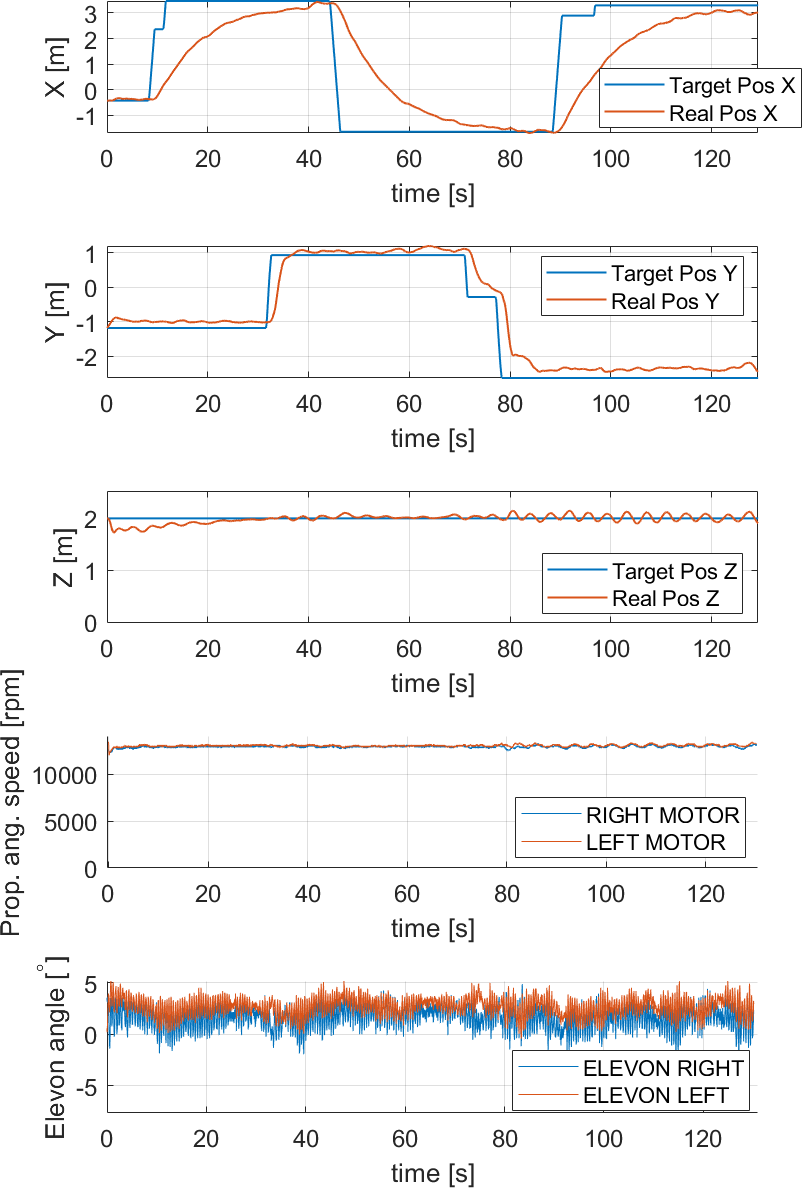
\includegraphics[width=0.6\columnwidth]{figures/realflight_z_adjust_x_adjust_final_HopeCrop.png}
   \vspace{-0.5cm}\caption{Réponse expérimentale en boucle fermée et entrée de commande pour $h = 12$.}
    \label{Dabbene_Flight_Test}
\end{figure}

Comme cela a également été observé dans les simulations, sur les axes $x$ et $z$, le temps de réponse est relativement élevée alors que sur l'axe $y$, il est plus rapide, en raison de l'actionnement différentiel important sur cet axe soutenu par la dynamique rapide de l'actionneur. 
% Sur l'axe $z$, le passage du contrôleur INDI au contrôleur synthétisé entraîne une descente verticale relativement importante du drone. Par conséquent, un réglage et une modélisation supplémentaire doivent être effectués afin de corriger les valeurs d'initialisation de l'état et de l'entrée de commande correspondant au point d'équilibre \eqref{eq:equilibria}.
 La dynamique du drone sur l'axe $z$ est caractérisée par de petites oscillations autour de la position de référence, qui peuvent également être observées dans le signal de commande des vitesses angulaires des hélices, illustré à la figure \ref{Dabbene_Flight_Test}. Ces oscillations réduites sont dues au fait que la dynamique de l'actionneur n'est pas prise en compte dans la loi de commande.
% Il convient de noter que l'objectif premier de l'algorithme d'optimisation est de parvenir à une stabilisation en boucle fermée, sans tenir compte des critères de performance ou de robustesse. 
Au cours des vols expérimentaux, le contrôleur n'a pas saturé les actionneurs (voir la figure \ref{Dabbene_Flight_Test}).



\section{Conclusion}

Pour traiter de la synthèse d'un retour statique de sortie, nous pouvons envisager deux approches étant donné le caractère non convexe et NP-difficile du problème. La première approche consiste à utiliser des outils d'optimisation non convexes pour directement optimiser les variables de décision du contrôleur, à savoir les matrices de gain. C'est ce qui est présenté dans le chapitre \ref{chap:3DOF} et \ref{chap:6DOF} en utilisant l'optimisation  non-lisse et la fonction {\tt Systune} de Matlab. La seconde approche consiste à utiliser des outils d'optimisation non convexe, ici l'outil LMI. Il s'agit alors de proposer un algorithme de résolution du problème BMI en une succession de problèmes LMI. C'est donc par exemple l'approche développe dans \cite{Arzelier2018} qui a été implémentée et testée en simulation et expérimentalement sur le drone. 

Un algorithme d'optimisation convexe, utilisant le cadre LMI et la théorie de la stabilité de Lyapunov, a été employé pour synthétiser des contrôleurs à retour de sortie statique pour le modèle de drone convertible DarkO. Cette technique de synthèse basée sur le modèle a permis de stabiliser efficacement la dynamique en boucle fermée du système, assurant une réponse temporelle satisfaisante et un suivi de la référence sans saturation des actionneurs. Malgré une prise en compte partielle des phénomènes non linéaires, les contrôleurs ont démontré un bon comportement lors des premiers tests expérimentaux sur le modèle de drone DarkO. Avec les matrices de gain du contrôleur conçues et la structure de la loi de commande, des vols expérimentaux ont été menés avec succès pour le vol stationnaire et le suivi de la trajectoire. Ce résultat constitue une solide preuve de concept pour la loi de commande développée en termes de performance.
Il est maintenant nécessaire de s'intéresser à l'impact du vent sur l'architecture du drone et aux impacts sur l'obtention des gains du contrôleur.
